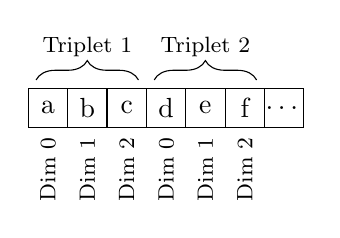
\begin{tikzpicture}

	% Rechtecke
	\draw (0,0) rectangle node {a} (0.5,0.5);
	\draw (0.5,0) rectangle node {b} (1,0.5);
	\draw (1,0) rectangle node {c} (1.5,0.5);
	\draw (1.5,0) rectangle node {d} (2,0.5);
	\draw (2,0) rectangle node {e} (2.5,0.5);
	\draw (2.5,0) rectangle node {f} (3,0.5);
	\draw (3,0) rectangle node {\ldots} (3.5,0.5);

	% Labels unten
	\foreach \x in {0, 1.5} {
		\draw (\x+0.25,0) node[left,rotate=90] {\footnotesize Dim 0};
		\draw (\x+0.75,0) node[left,rotate=90] {\footnotesize Dim 1};
		\draw (\x+1.25,0) node[left,rotate=90] {\footnotesize Dim 2};
	}

	% Klammern
	\draw [decorate,decoration={brace,amplitude=7pt},xshift=0pt,yshift=3pt]
		(0.1,0.5) -- (1.4,0.5) node[midway,yshift=12pt] {\footnotesize Triplet 1};
	\draw [decorate,decoration={brace,amplitude=7pt},xshift=0pt,yshift=3pt]
		(1.6,0.5) -- (2.9,0.5) node[midway,yshift=12pt] {\footnotesize Triplet 2};

\end{tikzpicture}
